\documentclass{article}
\usepackage{tikz}
\usepackage{pgfplots}
\usepackage{svg}
\usepackage{amsmath}
\usepackage{array}
\usepackage[skins]{tcolorbox}
\usepackage[version=4]{mhchem}
\usepackage[a4paper, total={6in, 9in}]{geometry}
\usepackage{fourier}
\usepackage{xymtex}
\usepackage{textcomp}
\usepackage{eurosym}
\usepackage{caption}
\usepackage{longtable}
\usepackage{float}
\usepackage{attachfile}
\usepackage{multirow}
\usepackage{amsfonts} 
\usepackage{tabularray}
\usepackage{colortbl}
\usepackage{xcolor}
\usepackage[table]{xcolor}
\UseTblrLibrary{booktabs}

\captionsetup[table]{name=Tabella}
\pagenumbering{gobble}
%\setcounter{secnumdepth}{2}


\renewcommand*\contentsname{Indice}
\setcounter{tocdepth}{3}
\setcounter{secnumdepth}{2}
\pgfplotsset{compat=1.15}


\title{Relazione di laboratorio - Esperienza di Poisson}
\author{Federico Cesari}
\date{Marzo 2024}




\begin{document}
\begin{titlepage}
   \begin{center}
       \vspace*{1cm}
        
       \textbf{\LARGE Relazione di laboratorio - Esperienza di Poisson}
       
       \vspace{0.3cm}
       \large \textit{Rate di una sorgente radioattiva} \\
       
       \vspace{0.5cm}
       \Large Federico Cesari \\
       
       \small 1096759

			
		\vspace{1cm}
		\begin{center}
			\includegraphics[scale=1.2]{geiger.jpeg}	
		\end{center}
		
		

       \vfill
            
       
            
       \vspace{0.8cm}
     
       
            
       corso A\\
       Università degli studi di Torino, Torino\\
       3 marzo 2024\\
       
            
   \end{center}
\end{titlepage}

\tableofcontents

\newpage
\textcolor{white}{.}
\vfill


\section{Scopo dell’esperienza}
\section{Premesse teoriche}
\section{Scelta strumento di misura}

Al fine di stabilire il migliore strumento di misura per le succesive misurazioni, registro 8 misure del periodo del pendolo prima con un angolo di partenza $\vartheta = 5^\circ$ e poi con $\vartheta = 30^\circ$ utilizzando un cronometro analogico, uno digitale e una fotocellula. Lo strumento che mostrerà discrepanze significative tra il periodo calcolato con $\vartheta = 5^\circ$ e $\vartheta = 30^\circ$ sarà quello utilizzato per i testi successivi.





\begin{minipage}[c]{0.3\textwidth}

\end{minipage}
\begin{minipage}[r]{0.7\textwidth}
\begin{table}[H]
	\centering
	\begin{tabular}{@{}lrrr@{}}
		&\textbf{C.Analogico} & \textbf{C. Digitale} & \textbf{Fotocellula} \\ \cmidrule(l){2-4} &\multicolumn{1}{l}{$T(s) \pm 0.2s$} & \multicolumn{1}{l}{$T(s) \pm 0.01s$}   & \multicolumn{1}{l}{$T(s) \pm 0.001s$}    \\ \cmidrule(l){2-4} 
		
		\multicolumn{1}{c}{}  
								& 1.6   & 1.63   & 1.702     \\
		\colorbox{orange!40}{$\vartheta = 5^\circ$}   & 1.7   & 1.65   & 1.703     \\
								& 1.5   & 1.60   & 1.703     \\ 
								& 1.7   & 1.71   & 1.703     \\
								& 1.7   & 1.71   & 1.703     \\
								& 1.7   & 1.65   & 1.702     \\
								& 1.6   & 1.70   & 1.703     \\
								& 1.7   & 1.70   & 1.703     \\ \arrayrulecolor{black!100}\specialrule{1.2pt}{0.5\jot}{0.5pc}
		
		$\mathbf{\bar{T}(s)}$ & \textbf{1.65}    & \textbf{1.67}  & \textbf{1.703}  \\
		$\sigma_{\bar{T}}$   & 0.05    & 0.02  & 0.000 \\                          
	\end{tabular}
\end{table}

\begin{table}[H]
	\centering
	\begin{tabular}{@{}lrrr@{}}
		&\textbf{C.Analogico} & \textbf{C. Digitale} & \textbf{Fotocellula} \\ \cmidrule(l){2-4} &\multicolumn{1}{l}{$T(s) \pm 0.2s$} & \multicolumn{1}{l}{$T(s) \pm 0.01s$}   & \multicolumn{1}{l}{$T(s) \pm 0.001s$}    \\ \cmidrule(l){2-4} 
		
		\multicolumn{1}{c}{}  
													& 1.8   & 1.65   & 1.733     \\
		\colorbox{blue!40}{$\vartheta = 30^\circ$}  & 1.7   & 1.67   & 1.733     \\
													& 1.6   & 1.70   & 1.733     \\ 
													& 1.7   & 1.62   & 1.733     \\
													
													& 1.7   & 1.70   & 1.731     \\
													& 1.8   & 1.72   & 1.733     \\
													& 1.7   & 1.80   & 1.733     \\
													& 1.6   & 1.69   & 1.732     \\ \arrayrulecolor{black!100}\specialrule{1.2pt}{0.5\jot}{0.5pc}

		$\mathbf{\bar{T}(s)}$ & \textbf{1.70}    & \textbf{1.69}  & \textbf{1.715}  \\
		$\sigma_ {\bar{T}}$   & 0.08    & 0.03  & 0.0005 \\                          
	\end{tabular}
\end{table}
\end{minipage}

Ora 


%%%%%%%%%%%%%%%%%%%%%%%%%%%%%%%%%%%%%%%%%%%%%%%%%%%%%%%%%
%%				DIPENDENZA THETA
%%%%%%%%%%%%%%%%%%%%%%%%%%%%%%%%%%%%%%%%%%%%%%%%%%%%%%%%%

\section{Dipendenza dall’angolo}



\begin{figure}[H]
	\centering
	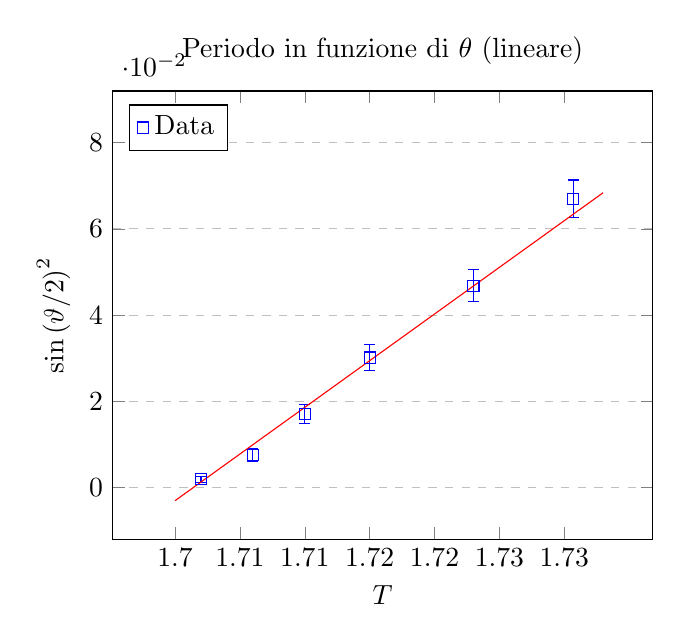
\begin{tikzpicture}
		\begin{axis}[
			title={Periodo in funzione di $\theta$ (lineare)},
			xlabel={$T$},
			ylabel={$\sin{\left( \vartheta / 2\right) }^2$},
			xmin=1.7, xmax=1.732,
			ymin=0, ymax=0.08,
			xtick={1.7,1.705,1.71,1.715,1.72,1.725,1.73},
			ytick={0,0.02,0.04,0.06,0.08},
			legend pos=north west,
			ymajorgrids=true,
			grid style=dashed,
			enlargelimits=0.15,
			]
			
			\addplot[
			only marks,
			color=blue,
			mark=square,
			error bars/.cd,
			y dir=both, y explicit
			]
			coordinates {
				(1.702,0.0019027) +- (0,0.00075825)
				(1.706,0.0075961) +- (0,0.00151074)
				(1.710,0.0170371) +- (0,0.00225173)
				(1.715,0.0301537) +- (0,0.00297558)
				(1.723,0.0468461) +- (0,0.00367678)
				(1.7307,0.0669873) +- (0,0.00435)
			};
			\addplot[
				domain=1.7:1.733, 
				samples=100, 
				color=red, 
				] 
				{2.16490*x -3.68337};
			\legend{Data}
		\end{axis}
	\end{tikzpicture}
	\caption{$T\left( \sin{\left( \vartheta / 2\right) }^2\right) $}
\end{figure}


\begin{figure}[H]
	\centering
	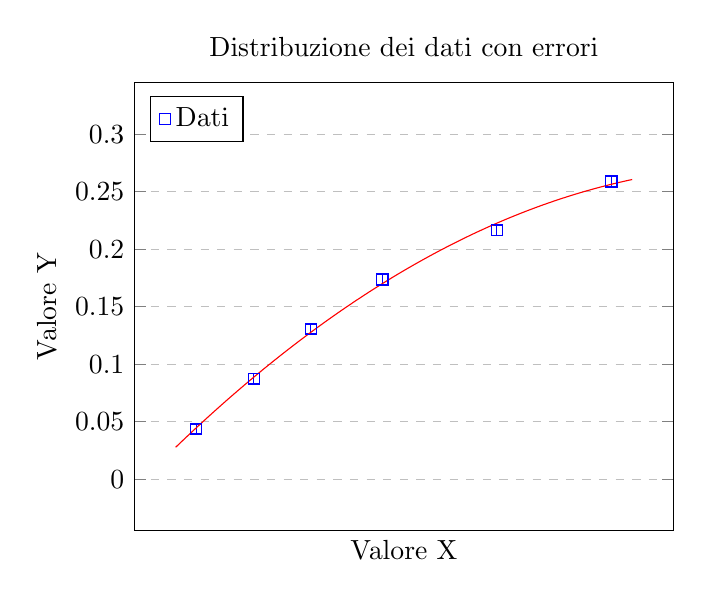
\begin{tikzpicture}
		\begin{axis}[
			title={Distribuzione dei dati con errori},
			xlabel={Valore X},
			ylabel={Valore Y},
			xmin=-1, xmax=1,
			ymin=0, ymax=0.3,
			xtick={1.7,1.71,1.72,1.73,1.74},
			ytick={0,0.05,0.1,0.15,0.2,0.25,0.3},
			tick label style={/pgf/number format/fixed},
			legend pos=north west,
			ymajorgrids=true,
			grid style=dashed,
			enlargelimits=0.15,
			]
			
			\addplot[
			only marks,
			mark=square,
			color=blue,
			error bars/.cd,
			y dir=both, y explicit
			]
			coordinates {
				(-1,0.0436194) +- (0,0.0086917/2)
				(-0.7241,0.0871557) +- (0,0.0086669/2)
				(-0.4482,0.1305262) +- (0,0.0086256/2)
				(-0.10344,0.1736482) +- (0,0.0085678/2)
				(0.4482,0.2164396) +- (0,0.0084938/2)
				(1,0.2588190) +- (0,0.0084036/2)
			};
			\addplot[
			domain=-1.1:1.1, 
			samples=100, 
			color=red, 
			] 
			{-0.03080*x^2 + 0.105900*x + 0.18138};
			\legend{Dati}
		\end{axis}
	\end{tikzpicture}
	\caption{Rappresentazione grafica dei dati sperimentali con errori ridotti.}
\end{figure}

\subsection{Confronto parametri parabola}

\subsection{g}

Calcolo il valore di g:
\[
T_0 = 2\pi\sqrt{\frac{l}{g}} \qquad \to \qquad T_0^2 = 4\pi^2\frac{l}{g}
\] 
\[
g = \frac{4l\pi^2}{T_0^2}
\]

poiché sappiamo che

\[
T = T_0 + \frac{T_0}{4}y \qquad \to \qquad y = 4\frac{T-T_0}{T_0} \qquad \to \qquad y = 4\frac{T}{T_0} - 4
\]
\[
b = \frac{4}{T_0} \qquad \to \qquad T_0 = \frac{4}{b}
\]

Quindi

\[
\mathbf{g = \frac{l\pi^2}{4}b^2}
\]

Calcolo l'errore associato a g:
\[
\sigma_g = \sqrt{\left(\frac{\partial g}{\partial l} \right)^2\sigma_l^2 + \left(\frac{\partial g}{\partial b} \right)^2 \sigma_b^2}
\]
\[
\sigma_g = 	\sqrt{\left(\frac{b^2\pi^2}{4}\right)^2 \sigma_l^2 + \left( \frac{lb\pi^2}{2}  \right)^2 \sigma_b^2	 }
\]

\subsubsection{Test Z per g}

Ottengo $g = ...$ ... Scelgo livello di significatività = 0.05.



\section{Dipendenza dalla lunghezza}

\begin{figure}[H]
	\centering
	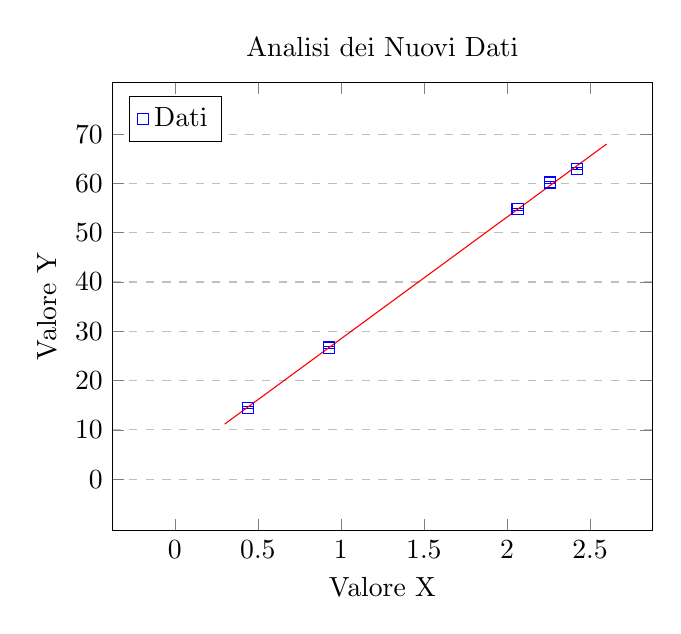
\begin{tikzpicture}
		\begin{axis}[
			title={Analisi dei Nuovi Dati},
			xlabel={Valore X},
			ylabel={Valore Y},
			xmin=0, xmax=2.5,
			ymin=0, ymax=70,
			xtick={0,0.5,1,1.5,2,2.5},
			ytick={0,10,20,30,40,50,60,70},
			legend pos=north west,
			ymajorgrids=true,
			grid style=dashed,
			enlargelimits=0.15,
			]
			
			\addplot[
			only marks,
			color=blue,
			mark=square,
			error bars/.cd,
			y dir=both, y explicit
			]
			coordinates {
				(2.260011111,60.20) +- (0,0.2)
				(0.9267271111,26.70) +- (0,0.2)
				(0.4391271111,14.50) +- (0,0.2)
				(2.422173444,63.00) +- (0,0.2)
				(2.064011111,54.80) +- (0,0.2)
			};
			\addplot[
			domain=0.3:2.6, 
			samples=100, 
			color=red, 
			] 
			{ 24.7131*x + 3.74511};
			\legend{Dati}
		\end{axis}
	\end{tikzpicture}
	\caption{Rappresentazione grafica dei dati sperimentali con errori.}
\end{figure}


\subsection{Confronto parametri retta}

\section{Dipendenza dalla massa}


\section{Conclusioni}



\end{document}
